\documentclass[11pt,a4paper,svgnames]{article}
\usepackage[english]{babel}
\usepackage{fontspec}
\usepackage{luacode}
\usepackage{fancyhdr}
\usepackage{relsize}
%https://tex.stackexchange.com/a/8633/42406
\usepackage{float}
%\usepackage[useregional]{datetime2}
%see https://tex.stackexchange.com/a/317859/42406
%\usepackage[utf8]{luainputenc}
%see https://tex.stackexchange.com/a/29594/42406
\usepackage{titling}
\usepackage[T1]{fontenc}
%\usepackage{xcolor}
\usepackage{hyperref}
%\usepackage{alltt}
%\usepackage{wasysym}
\usepackage{xcolor}
\usepackage{times}
%\usepackage[square]{natbib}
\usepackage{textcomp}
\usepackage{graphicx}
\usepackage{setspace}
\usepackage[backend=biber,bibencoding=utf8]{biblatex}
\addbibresource{../bib-refpersys.bib}
\usepackage[a4paper, margin=4cm]{geometry}
\setstretch{1.2}
\date{october 2019}
\newcommand*{\ac}[1]{\mbox{#1}}
\tolerance=600

\begin{luacode*}
  local gitpip=io.popen("git log --no-color --format=oneline -1 --abbrev=16 --abbrev-commit -q | cut -d' ' -f1")
  gitid=gitpip:read()
  gitpip:close()
  docdatetime = os.date('%Y-%b-%d %H:%M %Z')
  docdate = os.date('%Y-%b-%d')
\end{luacode*}
\newcommand{\mygitid}{\luadirect{tex.print(gitid)}}
\newcommand{\mydatetime}{\luadirect{tex.print(docdatetime)}}
\newcommand{\mydate}{\luadirect{tex.print(docdate)}}
\newcommand{\RefPerSys}{{\textit{\textsc{RefPerSys}}}}

 % see https://tex.stackexchange.com/a/51349/42406
\hypersetup{
  colorlinks   = true, %Colours links instead of ugly boxes
  urlcolor     = NavyBlue, %Colour for external hyperlinks
  linkcolor    = DarkGreen, %Colour of internal links
  citecolor   = DarkMagenta, %Colour of citations
  frenchlinks = true,
}
\setlength{\droptitle}{-10em}   % This is your set screw

\pagestyle{fancy}
\fancyhf{}
\rhead{\textit{\textsc{RefPerSys}} high-level goals and design ideas}
\fancyfoot[L]{{\raisebox{0.0cm}[1pt][1pt]{\color{LightSlateGrey}{{\relsize{+1}{DRAFT}}}~\relsize{-1.5}{\texttt{\mygitid} on \textit{\mydate}}}}}
\fancyfoot[R]{{Page \thepage}}
\begin{document}
\title {\textit{\textsc{RefPerSys}} high-level goals and design
  ideas\thanks{This document has git commit \texttt{\mygitid},
    was Lua-{\LaTeX} generated on \textit{\mydatetime}, see
    \href{http://gitlab.com/bstarynk/refpersys}{\texttt{gitlab.com/bstarynk/refpersys/}}
    and its \texttt{doc/design-ideas} subdirectory. Its draft is downloadable, as a \href{https://en.wikipedia.org/wiki/PDF}{PDF} file, from \href{http://starynkevitch.net/Basile/refpersys-design.pdf}{\texttt{starynkevitch.net/Basile/refpersys-design.pdf}} \ldots}}
\author {Basile
  \textsc{Starynkevitch}\thanks{See
    \href{http://starynkevitch.net/Basile/}{\texttt{starynkevitch.net/Basile/}}
    and contact
    \href{mailto:basile@starynkevitch.net}{\texttt{basile@starynkevitch.net}},
    92340 Bourg La Reine {\relsize{-1}(near Paris)}, France.}}

\begin{titlepage}
  \thispagestyle{empty}
  \maketitle

  \bigskip

  \begin{abstract}
    \textit{\textsc{RefPerSys}} is a \textsc{\textbf{Ref}}lexive and
    orthogonally \textsc{\textbf{Per}}sistent \textsc{\textbf{Sys}}tem
    (as a GPLv3+ licensed free software\footnote{Some code is
    available on
    \href{https://gitlab.com/bstarynk/refpersys}{\texttt{gitlab.com/bstarynk/refpersys}}.})
    running on Linux; it is a
    hobby\footnote{\href{http://starynkevitch.net/Basile/}{Basile
      Starynkevitch} (France) wants to find some research grant
    funding related to this. Please mention potential funding
    opportunities (call for research project proposals) by email to
    \href{mailto:basile@starynkevitch.net}{\texttt{basile@starynkevitch.net}}.} but serious \textbf{research project}
    for many years, mostly aimed to experiment \textbf{open science}
    ideas close to
    {AGI}\footnote{{\href{https://en.wikipedia.org/wiki/Artificial\_general\_intelligence}{Artificial
        General Intelligence}}} dreams, and we don't expect useful or
    interesting results before several years of hard work.
  \end{abstract}

  \medskip

  \textbf{audience :} \textsc{Linux} free software
  developers\footnote{Those \textsc{Linux} software developers are
  routinely \emph{glancing inside}, \emph{building} then using -from
  their published source code- quite large open source programs (such
  as \href{http://gcc.gnu.org/}{\textsc{Gcc}},
  \href{http://sbcl.org/}{\textsc{Sbcl}},
  \href{https://www.call-cc.org/}{\textsc{Chicken-Scheme}},
  \href{http://hop.inria.fr/}{\textsc{Hop}},
  \href{https://haxe.org/}{\textsc{Haxe}},
  \href{https://ocsigen.org}{\textsc{Ocsigen}},
  \href{https://www.gnu.org/software/emacs/}{\textsc{Emacs}},
  \href{https://sqlite.org/}{\textsc{Sqlite}},
  \href{https://mariadb.org/}{\textsc{MariaDb}}, etc...)  and perhaps
  even contributing to smaller free software projects like
  \href{https://ninja-build.org/}{\textsc{Ninja}},
  \href{https://github.com/davidmoreno/onion}{\texttt{libonion}},
  etc... By the way, all these open source projects could be useful to
  or inspirational for \RefPerSys.} and computer scientists interested in
  an experimental open science approach to reflexive systems,
  orthogonal persistence, symbolic artificial intelligence, knowledge
  engines, etc....


  \medskip
  \textbf{Nota Bene:} this report contains
  \href{https://en.wikipedia.org/wiki/Hyperlink}{hyperlinks} so its
  \href{https://en.wikipedia.org/wiki/PDF}{PDF} should rather be read
  on a computer screen, e.g. with
  \href{https://en.wikipedia.org/wiki/Evince}{\texttt{evince}}. Since
  it describes a circular design (with many
  \href{https://en.wikipedia.org/wiki/Cycle_graph}{cycles}
  \cite{Hofstadter:1979:GEB}), we recommend to read it twice (skipping
  footnotes and references on the first read).

  \bigskip


  \begin{quote}
  \begin{relsize}{-1}
  \includegraphics[width=75pt]{CC-BY-SA-icon} This entire document is
  licensed under the Creative Commons Attribution-ShareAlike 4.0
  International License. To view a copy of this license, visit
  \href{http://creativecommons.org/licenses/by-sa/4.0/}{\texttt{creativecommons.org/licenses/by-sa/4.0/}}
  or send a letter to Creative Commons, PO Box 1866, Mountain View, CA
  94042, USA.
  \end{relsize}
  \end{quote}
  
\end{titlepage}



\tableofcontents

\bigskip


\section{social necessity of \href{https://en.wikipedia.org/wiki/Artificial_general_intelligence}{AGI} systems with a long term development}
\label{sec:social}

\textbf{A}rtificial \textbf{G}eneral \textbf{I}ntelligence
(\emph{AGI}) systems are increasingly needed in our complex, but
fragile, world facing dramatic and extremely complex planet-wide
challenges (global warming, demographic and democratic or political
crisis, economical concerns, financial crisis, and increasing
inequalities).

As the very progressive and slow (but Darwinian) evolution of human
intelligence shows, our (limited) intelligence (as the
\emph{\href{https://fr.wikipedia.org/wiki/Homo_sapiens}{Homo Sapiens}
  Sapiens}\footnote{In latin, that means ``the human who knows what
  he/she knows'' and interestingly relates to both meta-knowledge and
  reflectivity.}  species) took more than a million years (so about 30
thousands generations) to progressively evolve from a monkey-like
state.

We don't believe in a single and simple model of intelligence. Any AGI
software system should be very complex. Inspired by observing huuman
natural intelligence (which is not yet understood and not yet
modelled\footnote{Despite the European taxpayer spending half a
  billion euro on the \href{https://www.humanbrainproject.eu}{Human
    Brain Project}; which did not produce a complete reproducible
  working artificial model of the human intelligence, but of course
  did fund interesting and quite successful research!}), we suppose
that any AGI system needs obviously to have a very complex and
self-improving organization.

We are aware than any progress towards AGI will be slow (many years,
perhaps decades\footnote{An interesting parallel could be controlled
  nuclear fusion -which also bears some ``bootstrrapping'' concepts-
  with \href{https://en.wikipedia.org/wiki/ITER}{\textsc{Iter}}; we
  expect {\RefPerSys} to cost several thousand times less at least;
  but even partial AGI success is as important for humanity as nuclear
  fusion produced electricity, and a future {\RefPerSys} might even
  help that \textsc{Iter}
  \href{https://en.wikipedia.org/wiki/Megaproject}{megaproject} or
  other ones.) and progressive. Remember
  \href{https://en.wikipedia.org/wiki/Hofstadter's_law}{Hofstadter's
    Law}: \textit{``It always takes longer than you expect, even when
    you take into account Hofstadter's Law''}
  \cite{Hofstadter:1979:GEB} and Brook's observations
  \cite{Brooks:1987:NSB, Brooks:1995:MM} that ``if one women can give
  birth in 9 months, 9 women cannot five birth toi a baby in one
  month''. For ``giving birth'' to {\RefPerSys}, a small team could
  need at least 9 years. However, intermediate results or side effects
  are not predictable but could be useful even during the {\RefPerSys}
  project.

We believe in free software (read also
\href{https://www.fsf.org/about/what-is-free-software}{this}), and we
strongly believe that an AGI prototype should be some free software,
exactly like most infrastructure software are (notably
\textsc{Linux}). See also the
\href{https://www.softwareheritage.org/}{\textsc{Software Heritage}
  project} for interesting insights. \textsc{RefPerSys} wants to be an
AGI infrastructure, and there is work for many years (several years of
work needed without any ``artificial intelligence'', just for the
infrastructure).


An even partially successful \textsc{AGI} system might be useful too
coordinate other existing software (described thru some knowledge
given declaratively). Imagine how complex future
\href{https://en.wikipedia.org/wiki/Digital_twin}{digital twins} of
the entire Earth planet, designed to tackle with global warming, would
need to be. For such dramatically complex usage, an AGI system (like
{\RefPerSys}, if we succeed in making it) could be quite helpful to
just drive and use such a ``digital twin'' simulation. Making it free
software runnable on a free software operating system should benefit
to most of humanity (but keeping it proprietary won't), and enable
further or alternative experimentations. And
``\href{https://theresnoplanetb.net/}{there is no planet
  B}''\footnote{As reminded E.Macron, president of France,
  \href{https://www.bbc.com/news/av/world-us-canada-43900009/macron-to-us-congress-there-is-no-planet-b}{to
    the US Congress}.}. So investing a few persons willing to working
for nearly a decade is not too much for such a perspective.


\section{\textsc{RefPerSys} ambitions and goals}
\label{sec:ambitions-goals}


\subsection{\textsc{RefPerSys} core idea{\texttt{[\textit{l}]\textsuperscript{?}}}s}
\label{subsec:coreidea}

The title of this subsection is \emph{not} a typo\footnote{It is a
geeky pun on words with
\href{https://en.wikipedia.org/wiki/Unix_shell}{shell}
\href{https://en.wikipedia.org/wiki/Glob_(programming)}{globbing} and
\href{https://en.wikipedia.org/wiki/Regular\_expression}{regexpr} like
syntax.}. We indeed mean both \textit{ideas} (that is, software design
and architectural concepts, guiding our daily implementation efforts)
and \textit{ideals} (that is, long term research objectives and
ambitions).

The \RefPerSys\footnote{For a \textbf{Ref}lexive \textbf{Per}sistent
  \textbf{Sys}tem}~ system shares several -but not all- goals and
design ideas (but no code) with
\href{http://github.com/bstarynk/bismon}{\texttt{bismon}}
\cite{Starynkevitch:2019:bismon-draft} but of course \emph{not}
\texttt{bismon}'s application\footnote{I Basile am not allowed and not
  funded to directly work on
  \href{https://en.wikipedia.org/wiki/Artificial_general_intelligence}{AGI}
  -which still is my major personal scientific interest- but I do get
  funded on applied research projects like
  \href{https://www.decoder-project.eu/}{\textsc{Decoder}} and try to
  push some AGI ideas into them.} to
\href{https://en.wikipedia.org/wiki/Static_program_analysis}{static
  source code analysis}. Like \texttt{bismon}, {\RefPerSys} is a
\textbf{reflexive} (it uses
\href{https://en.wikipedia.org/wiki/Reflection_(computer_programming)}{reflection}),
\textbf{\href{https://en.wikipedia.org/wiki/Virtual\_machine\_introspection}{introspective}}
and \textbf{orthogonally
  \href{https://en.wikipedia.org/wiki/Persistence_(computer_science)}{persistent}}
system, but not for
\href{https://en.wikipedia.org/wiki/Static_program_analysis}{static
  program analysis}. Please read Bismon's draft report
\cite{Starynkevitch:2019:bismon-draft} for a more precise definition
of these concepts. \textbf{\RefPerSys~ is a long term\footnote{I don't
    expect any significant AGI research results before $\approx
    2026$.}  risky
  \href{https://en.wikipedia.org/wiki/Research}{research} project with
  an \href{https://en.wikipedia.org/wiki/Open_science}{open science}
  mindset and
  \href{https://ropensci.github.io/reproducibility-guide/sections/introduction/}{reproducible
    experiment} ethics \cite{zuboff:2015:big-other,
    oneil:2016:weapons}, and a
  \href{https://www.gnu.org/philosophy/free-sw.en.html}{free software}
  licensed under
  \href{https://www.gnu.org/licenses/gpl-3.0.html}{GPLv3+}, and
  targetted \emph{only} for \textsc{Linux x86-64} computers.}. A Linux
system\footnote{My own \texttt{ours.starynkevitch.net} computer,
  running \textit{Debian/Unstable}, has 64 Gibytes of RAM, 24 cores
  (AMD 2970WX) and terabytes of disk space, including a terabyte of
  SSD.}  with at least 16 Gibytes of RAM, 4 \textit{x86-64} cores, and
220 Gibytes of disk is required. The grand ambition of {\RefPerSys} is
to become later an infrastructure for some strong
\href{https://en.wikipedia.org/wiki/Artificial_general_intelligence}{AGI}
system à la \textsc{Caia}\footnote{With explicit permission from
  J.Pitrat, \textsc{Caia} source code -entirely generated by itself,
  about half a million lines of C code- is available on
  \href{http://starynkevitch.net/Basile/}{my (Basile's) web page} as
  \href{http://starynkevitch.net/Basile/caia-su-24feb2016.tar.bz2}{\texttt{caia-su-24feb2016.tar.bz2}},
  and you could build it with \texttt{gcc -O -g [A-Z]*.c -rdynamic
    -ldl} then run \texttt{./a.out}. However, since I Basile sadly
  failed to convince J.Pitrat that open source
  \cite{Lerner-Tirole:2000:economics-open-source,
    Weber:2004:SuccessOpenSource} software are -in our
  XXI\textsuperscript{th} century- also an important way to transmit
  research ideas, there are no complete instructions to use it. Hence
  \textsc{Caia} has an undocumented user interface as user-friendly as
  the one of \href{https://www.gnu.org/software/ed/}{\texttt{ed}} but
  convenient enough to J.Pitrat alone! If you are capable of reading
  some comments in French and guessing the semantics of declarative
  ``expert system'' like rules (\textsc{Caia} has more than a dozen of
  thousands of them), run it, then type \texttt{L EDITE} and start
  reverse-engineering that brillant \textsc{Caia} system.}  by Jacques
Pitrat\footnote{Jacques Pitrat has passed away on October
  14\textsuperscript{th}, 2019. See quickly also his old web page on
  \href{http://jacques.pitrat.pagesperso-orange.fr/}{\texttt{jacques.pitrat.pagesperso-orange.fr}}
  and his interesting blog on
  \href{http://bootstrappingartificialintelligence.fr/WordPress3/}{\texttt{bootstrappingartificialintelligence.fr/WordPress3}}
  \ldots} \cite{Pitrat:1996:FGCS, Pitrat:2009:AST,
  Pitrat:2009:ArtifBeings}, but before even approaching that goal a
big lot of work is required, and {\RefPerSys} should be valuable by
itself for other less ambitious and more pragmatical purposes, perhaps
some specialized collaborative web server (GPLv3+) to ease
communication between human {\RefPerSys} developers, that is a mix of
a wiki, a chat, and a tool for sharing document with drawings or
graphics.

The development of {\RefPerSys} is (like the one of \texttt{bismon},
or
\href{http://bootstrappingartificialintelligence.fr/WordPress3/?s=CAIA}{of
  \textsc{Caia}}) a slow, incremental and gradual
\href{https://en.wikipedia.org/wiki/Bootstrapping}{bootstrapping}
process with a meta-programming \cite{dormoy:1992:meta} approach :
features added to {\RefPerSys} in January 2020 are used to implement
new features worked on a later {\RefPerSys} in March 2020.

As every practical software, {\RefPerSys} targets some defined
machines: common Linux distribution running on some
computer\footnote{For several years, that computer is a desktop or
powerful laptop running some \textsc{Debian}. Later that could be some
``virtual machine'' e.g. some
\href{https://www.docker.com/}{\textsc{Docker}} container.}. So the
target machine of {\RefPerSys} is a quite complete and modern Linux
system (such as a recent \textit{\textsc{Debian}} or
\textit{\textsc{Ubuntu}} desktop), with many useful packages, and
administred by some human person\footnote{For obvious cybersecurity
reasons, automatic administration of that Linux distribution is out of
scope. Also, since Basile Starynkevitch is still working (in october
2019) in a cybersecurity
\href{http://www-list.cea.fr/en/technological-research/research-programmes/embedded-systems/validation-and-verification}{lab}
(of about 25 permanent staff) at
\href{http://www-list.cea.fr/}{CEA/LIST}, cybersecurity concerns would
be a conflict of interest.}. The {\RefPerSys} system is published in
``source'' form, as a set of \href{http://git-scm.com/}{\texttt{git}}
versioned\footnote{We crucially depend upon \texttt{git}
\emph{specifically} (e.g. \href{http://gitlab.org/}{\texttt{gitlab}}),
and \href{https://en.wikipedia.org/wiki/Porting}{porting} {\RefPerSys}
to some other versioning system -or to some other
\href{http://pages.cs.wisc.edu/~remzi/OSTEP/}{operating system} than
\textsc{Linux}- would be a quite difficult task.} textual files
(e.g. \textit{C++} or \textit{C} files\footnote{However, notice that
bootstrapped language implementations like
\href{http://s48.org/}{Scheme 48} or \href{https://ocaml.org/}{Ocaml}
are keeping some
\href{https://en.wikipedia.org/wiki/Bytecode}{bytecode} form under
version control, and \href{https://www.call-cc.org/}{\textsc{Chicken
    Scheme}} is, like \texttt{bismon}, \texttt{git}-keeping generated
C files.}, perhaps some
\href{https://en.wikipedia.org/wiki/Makefile}{\texttt{Makefile}} or
better yet an
\href{http://projects.camlcity.org/projects/omake.html}{\textsc{Omake}}
build -most and more and more\footnote{Of course, in a
\href{https://en.wikipedia.org/wiki/Chicken_or_the_egg}{chicken and
  egg} fashion, the initial version of {\RefPerSys} has to contain
mostly hand-written files!} of them being generated- or shell files or
data files). Some of these files are generated, and the bootstrapping
goal is to have \emph{every} \texttt{git}-registered textual file been
generated by {\RefPerSys}, with a
\href{https://en.wikipedia.org/wiki/Bootstrapping\_(compilers)}{\textbf{bootstrap}ed}
approach\footnote{Observe that Linux source distributions like \href{http://www.linuxfromscratch.org/}{\texttt{linuxfromscratch.org}}, or to a lesser extent \href{https://www.gentoo.org/}{GenToo}, are also, when considered as a single system, fully bootstrapped.} similar to those of
\href{https://en.wikipedia.org/wiki/Self-hosting_(compilers)}{self-hosting
  compilers}.
\medskip

Within {\RefPerSys}, we call\footnote{Notice that, on purpose, our
terminology is different of usual habits in the open source realm:
almost all software projects (see also
\href{http://softwareheritage.org}{\texttt{softwareheritage.org}}) are
made of
\href{https://en.wikipedia.org/wiki/Computer\_file}{\textit{computer
    files}} typed by human developers in some
\href{https://en.wikipedia.org/wiki/Source-code\_editor}{source-code
  editor} or some
\href{https://en.wikipedia.org/wiki/Integrated\_development\_environment}{IDE}
such as \href{https://www.gnu.org/software/emacs/}{\texttt{emacs}},
\href{http://vim.org/}{\texttt{vim}} or
\href{http://codeblocks.org/}{\texttt{Code::Blocks}}, according to the
old \href{https://en.wikipedia.org/wiki/Unix\_philosophy}{Unix
  philosophy}. Notice that large open source projects like the
\href{https://www.libreoffice.org/}{\textsc{LibreOffice}} suite, the
\href{http://gcc.gnu.org}{\textsc{Gcc}} compiler collection or the
\href{https://www.mozilla.org/en-US/firefox/}{FireFox} browser tend to
accept
\href{https://en.wikipedia.org/wiki/Plug-in_(computing)}{plugins}
instead of favoring old fashioned
\href{https://en.wikipedia.org/wiki/Pipeline_(Unix)}{command
  pipelines}, but multi-threaded applications may follow the
\href{https://en.wikipedia.org/wiki/Pipeline_(software)}{pipeline
  design pattern}. In contrast, we are impatient to reach the state
where all {\RefPerSys} source files have been \texttt{git}-versioned
but are all generated by a previous run of our \texttt{refpersys}
executable. The {\RefPerSys} developer is interacting, thru a web
interface, with some running \texttt{refpersys} process, which is also some
specialized web server (using  HTTP).}  ``source file'' any Linux file which is
\texttt{git}-versioned. We hope that more and more of these source
files will be generated by the \texttt{refpersys}
\href{https://en.wikipedia.org/wiki/Executable\_and\_Linkable_Format}{ELF}
\href{https://en.wikipedia.org/wiki/Executable}{executable}
program. \textbf{A significant milestone is the entire bootstrapping
  of \RefPerSys}, when all files (in textual form, to stay
\texttt{git}-friendly, like
\href{https://en.wikipedia.org/wiki/Text-based_protocol}{text based
  protocols} are more friendly for developers) can be regenerated by
the \texttt{refpersys} executable, exactly in the same state as they
were previously\footnote{Pedantically, some
\href{https://en.wikipedia.org/wiki/Fixed\_point\_(mathematics)}{fixpoint}
of some very coarse-grained
\href{https://en.wikipedia.org/wiki/Operational\_semantics}{operational
  semantics} related to
\href{https://en.wikipedia.org/wiki/Abstract\_interpretation}{abstract
  interpretation} and
\href{https://en.wikipedia.org/wiki/Operational\_semantics\#Structural\_operational\_semantics}{big
  step semantics}, each big step being the entire regeneration of the
system, inspired by Futurama projections and
\href{https://en.wikipedia.org/wiki/Partial\_evaluation}{partial
  evaluation}.} : as a whole, our {\RefPerSys} system should become a
\href{https://en.wikipedia.org/wiki/Quine\_(computing)}{Quine
  program}, and \textsc{Caia} is already one. So the
\href{https://en.wikipedia.org/wiki/Build\_automation}{build
  automation} tool which compiles {\RefPerSys} should use file
contents, not modification times to trigger compilation commands,
since a full regeneration of such a bootstrapped {\RefPerSys} system
will touch all files, without changing the content of any of
them. Hence and very concretely, for building {\RefPerSys} the
\href{http://projects.camlcity.org/projects/omake.html}{\texttt{omake}}
build automation tool is preferable to \textsc{Gnu}
\href{https://www.gnu.org/software/make/}{\texttt{make}}.

For pragmatical reasons, \textbf{{\RefPerSys} needs a good
  \href{https://en.wikipedia.org/wiki/Tracing\_garbage\_collection}{garbage
    collector}} (or GC \cite{jones:2016:gchandbook}), since fully
compile-time GC \cite{mazur:2004:compile} are too difficult to
implement. Since multi-core x86-64 machines are very common, it should
take advantage of them, so \textbf{{\RefPerSys} should follow a
  \href{https://en.wikipedia.org/wiki/Thread_(computing)}{multi-threaded}
  approach} above \textsc{Posix} \cite{barney:2010:pthreads} or
\href{https://en.cppreference.com/w/cpp/thread}{C++11 threads}. Our GC
should be a
\href{https://en.wikipedia.org/wiki/Tracing_garbage_collection#Precise_vs._conservative_and_internal_pointers}{precise}
garbage collector \cite{Rafkind:2009:PreciseGC} and we may want to
favor, like what was done in \textsc{Gcc Melt}
\cite{Starynkevitch:2007:Multistage, Starynkevitch-DSL2011,
  Starynkevitch-GCCMELTweb}, fast allocation of small memory zones
which get quickly disposed of when becoming dead using a copying
generational
\href{https://en.wikipedia.org/wiki/Cheney's\_algorithm}{Cheney-like
  GC algorithm} \cite{wilson:1992:uniprocessorgc}.  But mixing
precise, sometimes generational GC techniques with multi-threading is
a difficult programming task. But precise-GC friendly programming is
simpler in generated C or C++ code that with hand-written code
(because of explicit management of local GC roots and write barriers,
à la
\href{http://starynkevitch.net/Basile/qishintro.html}{\textsc{Qish}}
or
\href{https://caml.inria.fr/pub/docs/manual-ocaml/intfc.html}{\textsc{Ocaml}}:
garbage collection invariants are boring and brittle to maintain in
hand-written code).


\href{https://en.wikipedia.org/wiki/Reification_(computer_science)}{Reification}
is an important concept in \RefPerSys, including (later) at the
\href{https://en.wikipedia.org/wiki/Knowledge_representation_and_reasoning}{knowledge
  representation} level with
\href{https://en.wikipedia.org/wiki/Semantic_network}{semantic
  networks} and
\href{https://en.wikipedia.org/wiki/Frame_(artificial_intelligence)}{frames}. {\RefPerSys}
\href{https://en.wikipedia.org/wiki/Call_stack}{call stacks} are made
of call frames known to our garbage collector (like
\href{https://caml.inria.fr/pub/docs/manual-ocaml/intfc.html}{\textsc{Ocaml}}'s
ones). They could later be copied into data structures representing
some
\href{https://en.wikipedia.org/wiki/Delimited_continuation}{delimited
  continuations} \cite{Reynolds:1993:continuations,
  Queinnec:2004:ContinWeb}, perhaps even representing and describing
control \cite{fouet-starynkevitch:describing-control:1987,
  Starynkevitch-1990-EUM, Pitrat:2009:ArtifBeings}. This should also
enable \textbf{introspection}, by permitting primitives inspecting the
current call stack, perhaps using Ian Taylor's
\href{https://github.com/ianlancetaylor/libbacktrace}{\texttt{libbacktrace}}.


{\RefPerSys} should (like \textsc{Caia} and its predecessor
\textsc{Malice} did
\cite{Pitrat:2009:AST,Pitrat:1996:FGCS,Pitrat:2009:ArtifBeings}) have
some expert system shell \cite{kumar:2015:importance-expert-systems,
  nigro:2008:meta} and meta-rules to ``dynamically compile'' some
subset of expert system rules and knowledge bases to procedural code
(e.g. with a metaprogramming approach of generating \emph{C} code, or
\href{https://gcc.gnu.org/onlinedocs/jit/}{\texttt{libgccjit}}
compiled code, then
\href{http://man7.org/linux/man-pages/man3/dlopen.3.html}{\texttt{dlopen(3)}}-ing
that code and running it at runtime. The
\href{https://github.com/bstarynk/misc-basile/blob/master/manydl.c}{\texttt{manydl.c}}
program show that this can practically be done many dozen of thousands
of times on Linux desktops).

{\RefPerSys} will extensively use
\href{https://en.wikipedia.org/wiki/Metaprogramming}{\textbf{metaprogramming}}
techniques, so it \textbf{should generate code} (like \textsc{Caia}
do) in a
\href{https://en.wikipedia.org/wiki/Source-to-source_compiler}{transpiler}
approach (in C, C++, -compiled into
\href{https://en.wikipedia.org/wiki/Plug-in\_(computing)}{plugins} and
later
\href{https://en.wikipedia.org/wiki/Dynamic\_loading}{dynamically
  loaded} with \href{}{\texttt{dlopen(3)}}- maybe also JavaScript and
HTML5 if we decide to have a web user interface). {\RefPerSys} could
also later use
\href{https://en.wikipedia.org/wiki/Just-in-time_compilation}{just-in-time
  compilation} libraries such as
\href{https://gcc.gnu.org/onlinedocs/jit/}{\texttt{libgccjit}}. The
domain-specific language of \RefPerSys\footnote{That domain-specific
language has to be defined and implemented in a bootstrapped manner.}
(a declarative one, with ``expert system rules'') should gradually
increase its expressiveness and become more and more declarative and
closer to mathematical formalisms.

Most Linux distributions contain lots of useful libraries or software
components for {\RefPerSys} long-term goals, notably machine learning
open source libraries like
\href{https://www.tensorflow.org/}{\textsc{TensorFlow}}
\cite{charniak:2019:deep-learning} or
\href{https://gudhi.inria.fr/}{\textsc{Gudhi}}
\cite{chazal:2016:high}. We might at some point also need messaging
libraries like \href{https://zeromq.org/}{\textsc{0mq}}, graphical
user interfaces libraries à la \href{http://qt.io/}{\textsc{Qt}} or
more probably web servicing libraries like
\href{https://github.com/davidmoreno/onion/}{\texttt{libonion}} or
\href{https://www.webtoolkit.eu/wt}{\textsc{Wt}}. To decrease efforts,
we don't want to rewrite such libraries inside {\RefPerSys} (considered
as a very high level,
\href{https://en.wikipedia.org/wiki/Declarative\_programming}{declarative},
\href{https://en.wikipedia.org/wiki/Domain-specific\_language}{domain-specific
  language}). Hence, we will need in {\RefPerSys} to generate some
glue code, like \href{http://swig.org/}{\textsc{Swig}} does, from some
\textbf{declarative description} (probably some frames or knowledge
bases) of the
\href{https://en.wikipedia.org/wiki/Application_programming_interface}{API}
of these available libraries.

{\RefPerSys} should at first be \textbf{orthogonally
  \href{https://en.wikipedia.org/wiki/Persistence\_(computer\_science)}{persistent}}. Like
\textsc{Bismon} \cite{Starynkevitch:2019:bismon-draft} it will load
its state (its entire garbage-collected
\href{https://en.wikipedia.org/wiki/Memory\_management#HEAP}{heap})
from files at startup, and will dump its state\footnote{In a manner
inspired by \textsc{Sbcl}
\href{http://www.sbcl.org/manual/index.html\#Saving-a-Core-Image}{\texttt{save-lisp-and-die}}
primitive, or \href{https://www.polyml.org/}{\textsc{PolyML}}
\href{https://www.polyml.org/documentation/Reference/PolyMLStructure.html\#export}{\texttt{export}}
primitive, or
\href{https://en.wikipedia.org/wiki/Marshalling_(computer_science)}{marshalling}
\href{https://caml.inria.fr/pub/docs/manual-ocaml/libref/Marshal.html}{facilities} of \textsc{Ocaml} or \textsc{Python}
\href{https://docs.python.org/3/library/pickle.html}{\texttt{pickle}}
module.} into files at shutdown. These state files are
textual\footnote{We should decide if we use some
\href{http://json.org/}{\textsc{Json}} or
\href{http://yaml.org/}{\textsc{Yaml}} notation, or our own one for
\RefPerSys.} and \texttt{git}-versioned, and should be portable to
other 64 bits Linux computers. A
\href{https://en.wikipedia.org/wiki/Manifest\_file}{manifest file}
describing the collection of files keeping the state is probably
needed.

\subsection{{\RefPerSys} strange development cycle}
\label{subsec:strange-devel}

Ordinary software projects tend to follow a spiral development model
\cite{boehm:1988:spiral} as shown in figure \ref{fig:tradspiral}.
%
\begin{figure}[h]
  \begin{center}
    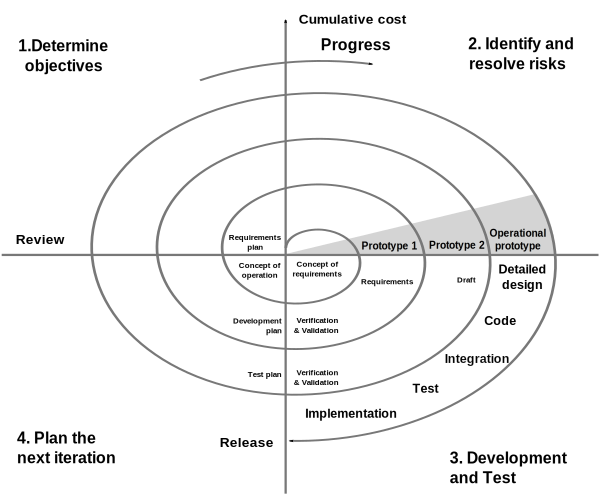
\includegraphics[width=0.8\textwidth]{spiral-model-softdevel}
  \end{center}
  \caption{the \textbf{traditional spiral development} model (from Wikipedia \href{https://en.wikipedia.org/wiki/Spiral_model}{spiral model})}
  \label{fig:tradspiral}
\end{figure}
%
But \RefPerSys' development follows a
\href{https://en.wikipedia.org/wiki/Strange_loop}{strange loop}
\cite{hofstadter:2007:strange-loop}, since it is bootstrapped in an
\href{https://en.wikipedia.org/wiki/Software\_prototyping\#Evolutionary\_prototyping}{evolutionary
  prototyping} manner. It is more like a spiral staircase like in
figure \ref{fig:bootstrap-stair}. The initial (floor) is just a
persistent system, and we gradually add new code implementing more
features (first entirely hand-written, later more and more parts of it
replaced by {\RefPerSys} generated code). Of course the fun is in
replacing existing hand-written code (or low-level DSL) by more
expressive and generated one. So we will continuously rewrite past
formalizations as a more clever and expressive ones, taking more and
more advantage of {\RefPerSys} whole-system introspective abilities.
All of \href{https://en.wikipedia.org/wiki/Eurisko}{\textsc{Eurisko}}
\cite{Lenat:1983:Eurisko},
\href{https://en.wikipedia.org/wiki/Cyc}{\textsc{Cyc}}
\cite{Lenat:1991:ev-cycl} and
\href{https://en.wikipedia.org/wiki/Self\_(programming_language)}{\textsc{Self}}\footnote{\textsc{Self}
was even able (in hours of CPU time) to redefines its integers -even
for arithmetic used inside its compiler- as
\href{https://en.wikipedia.org/wiki/Arbitrary-precision_arithmetic}{bignums}.}
\cite{chambers:1991:efficient} (or even
\href{https://iolanguage.org/}{\textsc{Io}} or
\href{https://en.wikipedia.org/wiki/Smalltalk}{\textsc{Smalltalk}})
systems and their incremental development process are inspirational.

\begin{figure}[h]
  \begin{center}
    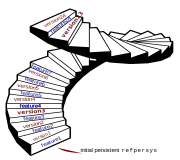
\includegraphics[width=0.8\textwidth]{spiral-stairs}
  \end{center}

  \begin{quote}
    \begin{relsize}{-0.2}
    Each new feature -or small incremental change or a few of them
    (small \texttt{git commit}s) - of {\RefPerSys} enables us to build
    and \textbf{generate} the next version of {\RefPerSys}, and a next
    feature is then added to that \textit{improved} version, and so on
    repeatedly, etc....
    \end{relsize}
  \end{quote}
  
  \caption{the strange \textbf{{\RefPerSys} staircase development model} {\relsize{-1}{(from a \href{https://thenounproject.com/term/spiral-stairs/956427/}{figure of Spiral stairs} by Lluisa Iborra from the Noun Project)}}}
  \label{fig:bootstrap-stair}
\end{figure}

\bigskip

\subsection{\textsc{RefPerSys} persistent heap}
\label{subsec:persistheap}

When {\RefPerSys} is running in some multi-threaded \textsc{Linux}
\href{https://en.wikipedia.org/wiki/Process\_(computing)}{process},
the {\RefPerSys} persistent heap is (like Bismon's one
\cite{Starynkevitch:2019:bismon-draft}) semantically like the memory
heap of most
\href{https://en.wikipedia.org/wiki/Dynamic\_programming\_language}{dynamic
  programming languages} (such as
\href{https://python.org/}{\textsc{Python}},
\href{https://www.gnu.org/software/guile/}{\textsc{Guile}},
\href{https://golang.org/}{\textsc{Go}},
\href{http://sbcl.org/}{\textsc{Sbcl}}, etc \ldots). The
%%\textcolor{red}{\textbf{\relsize{+1}{still incomplete}}}
figure \ref{fig:persistent-heap} should give an intuition about that
heap, when it is inside the
\href{https://en.wikipedia.org/wiki/Virtual_address_space}{virtual
  address space} of some \texttt{refpersys} process. We strongly want
to avoid any
\href{https://en.wikipedia.org/wiki/Global\_interpreter\_lock}{GIL},
but multi-threaded precise efficient garbage collector implementations
are quite difficult to code. However, notice that the persistence
(dump as textual \texttt{git}-versioned disk files) of a heap uses
algorithms similar to those of copying garbage collectors
\cite{wilson:1992:uniprocessorgc, jones:2016:gchandbook}.

\begin{figure}[H]
  \begin{center}
    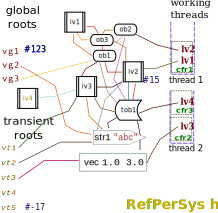
\includegraphics[width=0.8\textwidth]{heap-refpersys}
  \end{center}

\begin{quote}
  \begin{relsize}{-0.2}
    \begin{tabular}{ll}
      \texttt{\textbf{\textit{\#123}}} & a tagged 63 bits integer \\
      \texttt{\textit{vg1}} & a global persisted variable \\
      \texttt{\textit{vt2}} & a static transient variable \\
      \texttt{\textbf{ob1}} & a mutable persistent object \\
      \texttt{\textbf{iv2}} & an immutable constant composite value \\
      \texttt{\textbf{iv4}} & an immutable but \textbf{dead} constant composite value (should be GC-ed) \\
      \texttt{\textbf{tob1}} & a transient mutable object \\
      \texttt{str1} & a constant \textsc{utf-8} string value \texttt{"abc"} \\
      \texttt{vec} & a constant vector of floats {$ [1.0; 3.0] $} \\
      \texttt{\textit{lv2}} & a local variable inside its call frame \\
      \textit{cfr1} &  a \textbf{call frame} (simplified) \\
      \textit{\textbf{thread1}} & a \textbf{working thread} and its call stack (simplified) \\
    \end{tabular}
    \medskip

    In real life, the heap may be quite large (gigabytes) and contain
    hundreds of global roots or transient roots, millions of objects
    (sometimes transient, often persistent) and many millions
    immutable values (some of them composite and containing values,
    other scalar and containing non-pointer data like strings or
    vectors of float do), and dozen of working threads, each having
    thousands of call frames with dozens of local variables each.
   \end{relsize}
\end{quote}
  
  \caption{the  \textbf{{\RefPerSys} persistent heap}  (simplified)}
  \label{fig:persistent-heap}
\end{figure}

That figure \ref{fig:persistent-heap} shows a few global and transient
roots (both being processed by the garbage collector), and several
threads each having its call stack (made of call frames) with local
variables in it. The heap is actually a large directed graph and may
contain cycles (e.g. $ ob1 \rightarrow iv1 \rightarrow ob3 \rightarrow
ob2 \rightarrow ob3 $). Most values are immutable values (some of them
being composite, such as \texttt{iv1}). Some immutable values are
scalar (e.g. strings). Notice that \texttt{iv4} is a dead value,
unreachable from others; it should be later garbage collected.  Only
objects have a content which may change. Since {\RefPerSys} is
multi-threaded, the access inside every object should be thread-safe
and usually is protected by a \href{https://en.wikipedia.org/wiki/Lock\_(computer\_science)}{\textit{mutex}} (or \textit{read write
  lock}) which is part of that object\footnote{Or by atomic pointers,
probably the {\RefPerSys} class of an object is, inside it, given by
some C++ field with an
\href{https://en.cppreference.com/w/cpp/atomic/atomic}{\texttt{std::atomic}}
pointer type, for efficiency reasons.}.


Conceptually, {\RefPerSys}
\href{https://en.wikipedia.org/wiki/Tracing_garbage_collection}{tracing
  precise garbage collector} should traverse the graph of references
to {\RefPerSys} values, starting from global or transient roots and
local variables inside call frames of working threads. Each
{\RefPerSys} value (immutable or object) is represented by a machine
word (aligned, 64 bits) which usually contains a pointer, but
sometimes some
\href{https://en.wikipedia.org/wiki/Tagged\_pointer}{tagged integer}.
Immutable values are often ``small'' (a few dozens of words) but
objects are necessarily heavier since they contain some kind of
lock. \href{https://en.wikipedia.org/wiki/Closure\_(computer_programming)}{closures}
are immutable values, containing an object representing and giving
their function code (as a C function pointer inside that object), and
additional closed values.

Some values (or objects) are dead; in the figure
\ref{fig:persistent-heap}, the immutable value \texttt{iv4} is not
reachable from roots or local variables on the call stack of working
threads. So it is dead and should eventually be reclaimed by the
garbage collector.

\textbf{Values} -either immutable values or changeable objects- in
{\RefPerSys} can be either \textbf{persistent} (dumped in
textual state files\footnote{In the current implementation,
{\RefPerSys} state files and their manifest file should appear
under \texttt{persistore/} subdirectory.}, then reloaded at
restart of \texttt{refpersys} process) or \textbf{transient}
(that is, not dumped and not appearing in state files).

The \textbf{persistence} machinery - the dump - is conceptually simple
and could run in several threads: start from global roots and travers
the memory graph but ignore transient objects and transient roots and
memoize previously seen persistent objects. Of course, objects should
not be persisted twice, and are referred by the \textbf{object id} or
\textbf{oid} in the state files produced by the dump. That
\textit{oid} is alphanumeric, randomly generated and so hopefully
globally unique -like {\relsize{-1}{\texttt{\_2om48kc3k5R02d3ktW}}}
for example- in our current implementation; exactly like
\href{https://en.wikipedia.org/wiki/Universally_unique_identifier}{\textsc{Uuid}s}
should be. Notice the conceptual similarity between {\RefPerSys} dump
algorithm and its tracing garbage collector: both are traversing the
graph of references inside the heap.

The initial loading machinery (recreating a suitable heap - and
rebuilding a graph of references inspired by figure
\ref{fig:persistent-heap}, without any transient stuff) from its
previous dumped state) is first creating empty all objects, then later
filling each of them. However, for efficiency, we may want to load the
heap in parallel, using several loader threads. This could be easy if,
after having created all objects as empty, and loaded plugins
(i.e. \texttt{dlopen}-ing many \texttt{*.so} files), {\RefPerSys}
processes each state file in a potentially different loading thread.

\bigskip

\section{the data and object models of \RefPerSys}
\label{sec:dataobjmodel}

\subsection{how data should be processed in \RefPerSys}
\label{subsec:howdata}

{\RefPerSys} aiming to be first a good old fashioned AI system
(\href{http://bootstrappingartificialintelligence.fr/WordPress3/2013/12/the-future-of-ai-is-the-good-old-fashioned-artificial-intelligence/}{\textsc{Gofai}}),
better known as
\href{https://en.wikipedia.org/wiki/Symbolic\_artificial\_intelligence}{symbolic
  artificial intelligence} system, it is targetting mostly
\href{https://en.wikipedia.org/wiki/Computer\_algebra}{symbolic
  computation}, in particular using a
\href{https://en.wikipedia.org/wiki/Semantic\_network}{semantic
  network} or other forms of mathematical finite but large
\href{https://en.wikipedia.org/wiki/Graph\_(discrete\_mathematics)}{graph}
representations, in particular
\href{https://en.wikipedia.org/wiki/Abstract\_syntax\_tree}{abstract
  syntax trees}\footnote{Practically speaking, abstract syntax trees
are in fact at least finite
\href{https://en.wikipedia.org/wiki/Directed_acyclic_graph}{directed
  oriented graphs} and could even have cycles if you relate a
\href{https://en.wikipedia.org/wiki/Symbol\_(programming)}{symbol} to
its properties.} of generated programs, of internal rules or
expressions, by some internal metaprogramming machinery. So
{\RefPerSys}
\href{https://en.wikipedia.org/wiki/Object_(computer_science)}{objects}
should have a finite but changing set of
\href{https://en.wikipedia.org/wiki/Attribute_(computing)}{attributes}
or
\href{https://en.wikipedia.org/wiki/Property_(programming)}{properties}
and be organized, as in most
\href{https://en.wikipedia.org/wiki/Object-oriented_programming}{object-oriented
  languages}. Hence,
\href{https://en.wikipedia.org/wiki/Electronic\_document}{documents},
\href{https://en.wikipedia.org/wiki/Hypertext}{hypertext}, high-level
\href{https://en.wikipedia.org/wiki/Source\_code}{source code},
\href{https://en.wikipedia.org/wiki/Ontology\_(information\_science)}{ontologies},
\href{https://en.wikipedia.org/wiki/Knowledge\_base}{knowledge bases},
\href{https://en.wikipedia.org/wiki/Expert\_system}{expert systems},
implementation of some
\href{https://en.wikipedia.org/wiki/Inference_engine}{inference
  engine} guided by
\href{https://en.wiktionary.org/wiki/metarule}{metarules}, etc \ldots~
should all be easily and conveniently representable\footnote{So
\href{https://en.wikipedia.org/wiki/Artifact_(software_development)}{artifacts}
like \href{https://en.wikipedia.org/wiki/XML}{\textsc{Xml}} documents,
\href{https://en.wikipedia.org/wiki/HTML5}{\textsc{Html5}} or
\href{https://en.wikipedia.org/wiki/XHTML}{\textsc{Xhtml}} hypertexts,
\href{http://json.org/}{\textsc{Json}} data,
\href{https://yaml.org/}{\textsc{Yaml}} representations should all be
easily representable and inspirational for {\RefPerSys} data and its
processing.}  and processable, as some evolving subgraph of
{\RefPerSys} values.

Since {\RefPerSys} objects are the only mutable values, they keep not
only their synchronization data, but also attributes or properties,
components, and some extra payload. See also \S
\ref{subsec:mutable-objects} below.

The {\RefPerSys} worker threads, organized in a small
\href{https://en.wikipedia.org/wiki/Thread_pool}{thread
  pool}\footnote{Threads are heavy resources, each of them needing a
call stack and, practically speaking, a processor core to run. We
surely want to have at most a dozen of worker threads.} are somehow
organized in some
\href{https://en.wikipedia.org/wiki/Agenda}{\textbf{agenda}}\footnote{In
Latin, ``agenda'' means ``things which have to be done or
completed''.}  mechanism. Informally, the agenda is a clever
organization (perhaps a few mostly
\href{https://en.wikipedia.org/wiki/FIFO}{FIFO}
\href{https://en.wikipedia.org/wiki/Queue\_(abstract\_data\_type)}{queue}
of elementary tasklets, or something more complex). Each such tasklet
runs for a short time\footnote{In practice, several dozens of
milliseconds, to play nice with human interaction and be friendly with
our garbage collector} and may, while running, update that agenda by
adding further runnable tasklets to it, or by removing some of
them. The agenda itself should be somehow reified and partly
persistent, and tasklets are {\RefPerSys} objects. Of course some
tasklets (e.g. those directly related to the user interface,
e.g. \href{https://en.wikipedia.org/wiki/Ajax_(programming)}{\textsc{Ajax}}
or \href{http://qt.io/}{\textsc{Qt}} callbacks) are transient.

\label{subsec:datalowhigh}
\subsection{data at the low and high levels}
\label{subsec:datalowhigh}

{\RefPerSys} mostly handle values\footnote{In particular, only
\textsc{closures} are
\href{https://en.wikipedia.org/wiki/Function_application}{applied}, to
arguments which are values (read more about
\href{https://en.wikipedia.org/wiki/Lambda_calculus}{$\lambda$-calculus});
or messages are sent, to values with perhaps additional value
arguments.}, which can be either ``light'' immutable values or
  ``heavy'' mutable objects. Our data model is inspired by the
  \href{https://en.wikipedia.org/wiki/ObjVlisp}{\textsc{ObjVLisp}}
  model (or
  \href{https://en.wikipedia.org/wiki/Common_Lisp_Object_System}{\textsc{CLOS}},
  see also the
  \href{http://www.lispworks.com/documentation/HyperSpec/Front/index.htm}{Common
    Lisp HyperSpec}) common in most Lisp implementations
  \cite{queinnec:2003:lisp, cointe:1987:metaclasses,
    briot:1987:uniform} and inspired by
  \href{https://en.wikipedia.org/wiki/Smalltalk}{\textsc{Smalltalk}}
  \cite{kay:1996:early-smalltalk}. Also, a value can be transient or
  persistent. Each {\RefPerSys} value fits in one 64 bits machine
  word\footnote{Remember: {\RefPerSys} targets only Linux x86-64
  systems!}, so is nicely represented as a pointer or a tagged integer
  (63 bits, with the least significant bit being set to 1). Values are
  usually pointers to complex structures, so, per the
  \href{https://github.com/hjl-tools/x86-psABI/wiki/x86-64-psABI-1.0.pdf}{x86-64
    calling conventions}, are word aligned (address multiple of 8
  bytes). Let's call \emph{genuine values} those that are not
  \href{https://medium.com/@hinchman_amanda/null-pointer-references-the-billion-dollar-mistake-1e616534d485}{\texttt{null}}
  and not tagged pointers (so either immutable values or objects in
  figure \ref{fig:persistent-heap}). These genuine values are
  practically implemented as a \href{
    https://en.wikipedia.org/wiki/Tagged_union}{tagged
    union}\footnote{An old example of tagged unions in C is the
  \href{https://tronche.com/gui/x/xlib/events/structures.html}{X11
    event structure}, but
  \href{https://www.gnu.org/software/guile/manual/html\_node/A-Simple-Representation.html}{\textsc{Guile}}
  and
  \href{https://caml.inria.fr/pub/docs/manual-ocaml/intfc.html}{\textsc{Ocaml}}
  use similar implementation tricks.} and each of them start with a
  field (probably 16 bits) identifying their concrete type.

  For pragmatical reasons, our values should be both ordered and
  hashed, since many
  \href{https://en.wikipedia.org/wiki/Data\_structure}{data
    structures} \cite{cormen:2009:introduction}, specified as some
  \href{https://en.wikipedia.org/wiki/Abstract_data_type}{abstract
    data type}, either uses some ordering
  (e.g. in \href{https://en.wikipedia.org/wiki/Red-black_tree}{red-black
    trees}) or some hash-code (e.g. various kinds of
  \href{https://en.wikipedia.org/wiki/Hash_table}{hash
    tables}). Because of the weird and counter-intuitive semantics of
  \href{http://floating-point-gui.de}{floating point} numbers, the
  \href{https://en.wikipedia.org/wiki/NaN}{\textsc{NaN}} should be
  handled specifically (it is unordered), if we
  \href{https://en.wikipedia.org/wiki/Object\_type\_(object-oriented\_programming)\#Boxing}{box}
  IEEE \texttt{double}s.

\subsection{immutable values}
\label{subsec:immutable-values}

By definition, immutable values don't change. All their useful
bits\footnote{For housekeeping purposes, our garbage collector may
reserve a few bits, e.g. for
\href{https://www.memorymanagement.org/glossary/t.html}{tri-color}
marking \cite{wilson:1992:uniprocessorgc}} stay unchanged as long as
the value is alive. Some values are scalar (strings, vectors of
floats, perhaps bitmaps\footnote{In practice, bitmaps or pixmaps would
rather be the payload of some objects, see below.} if we reify
them). Other values are composite.

Since objects are fundamental, we want to keep finite collections of
them. In particular, {\RefPerSys} will reify (represent as first-class
values) \textbf{tuples} of objects and finite \textbf{sets} of objects
as values, and they are the common composite values of \RefPerSys. A
tuple is obviously represented by boxing a sequence of object
references (i.e. pointers). A set would be represented by an ordered
sequence of objects, with membership efficiently testable by a
\href{https://en.wikipedia.org/wiki/Time\_complexity}{$O(log~ n)$}
time
\href{https://en.wikipedia.org/wiki/Binary_search_algorithm}{binary
  search algorithm}). We expect most of tuples and sets to be small
and fitting in an
\href{https://en.wikipedia.org/wiki/Cache\_hierarchy}{L1 or L2 cache
  line}, so their processing should be efficient.

\textcolor{red}{@@TODO: should explain implementation details in C terms?}

\subsection{mutable objects}
\label{subsec:mutable-objects}

Practically speaking, mutable objects are heavy, since they should
carry inside them locking devices\footnote{At the implementation
level, think of some
\href{https://computing.llnl.gov/tutorials/pthreads/\#Mutexes}{mutex}
or
\href{http://tuxthink.blogspot.com/2013/02/using-read-write-lock-in-pthreads.html}{read-write
  lock, so
  \href{https://pubs.opengroup.org/onlinepubs/7908799/xsh/pthread\_mutex\_init.html}{\texttt{pthread\_mutex\_init}}
  or
  \href{https://pubs.opengroup.org/onlinepubs/7908799/xsh/pthread_rwlock_init.html}{\texttt{pthread\_rwlock\_init}}}
or \href{https://en.cppreference.com/w/cpp/thread}{C++11
  equivalents}.} for multi-threading support. And each object carries
an association between attributes (playing the role of arbitrary keys)
and their corresponding value. In addition, an object can carry its
payload\footnote{Every payload belongs to a single object, its owner!}
for stuff which does not fit into that model. For example, an object
may carry as its payload a dictionnary associating machine strings to
values, or an hash-table of triplets, or an opened \texttt{FILE*}
handle, or \href{https://en.wikipedia.org/wiki/File\_descriptor}{file
  descriptor}\footnote{\href{https://en.wikipedia.org/wiki/Finalizer}{Finalizers}
are practically not enough to handle these, even if they are useful,
in our GC, as a last resort mesure!}, or some
\href{https://www.tensorflow.org/}{\textsc{TensorFlow}} or
\href{https://gudhi.inria.fr/}{\textsc{Ghudi}} data for machine
learning purposes, maybe something related to
\href{https://github.com/davidmoreno/onion/}{\texttt{libonion}} or
\href{http://zeromq.org}{\texttt{0mq}}, some
\href{https://gmplib.org/}{\textsc{GMPlib}} big number, some
\href{https://www.bugseng.com/ppl}{\texttt{PPL}} polyhedra, maybe some
\href{http://qt.io/}{\textsc{Qt}} graphical widget, etc \ldots. Of
course every object has its class (which is itself an object, having a
\href{https://en.wikipedia.org/wiki/Metaclass}{metaclass}) and carries
a function pointer\footnote{That function pointer should be, for
efficiency reasons (we don't want to lock an object to get that
pointer!)
\href{https://en.cppreference.com/w/c/atomic}{\texttt{atomic}} in C
parlance, and might be set using
\href{http://man7.org/linux/man-pages/man3/dlsym.3.html}{\texttt{dlsym(3)}}.}.

Notice that a generational GC approach moving data is possible for
some immutable values, but not for objects and their optional payload,
since {\RefPerSys} objects contain locks and payloads that are dealt
with thru external functions requiring fixed, unchangeable, pointers.

\textcolor{red}{@@TODO: should explain a lot more}
\clearpage


\printbibliography

\end{document}

%%%%%%%%%%%%%%%%%%%%%%%%%%%%%%%%%%%%%%%%%%%%%%%%%%%%%%%%%%%%%%%%
%% Local Variables: ;;
%% compile-command: "./build.sh" ;;
%% End: ;;
%%%%%%%%%%%%%%%%%%%%%%%%%%%%%%%%%%%%%%%%%%%%%%%%%%%%%%%%%%%%%%%%
